\begin{enumerate}[label=\thesubsection.\arabic*.,ref=\thesubsection.\theenumi]
\numberwithin{equation}{enumi}

\item A second-order LTI system is described by the following state equations
\begin{align}
\label{:ee18btech11031_qe1}
\frac{\partial x_1(t)}{\partial t} - x_2(t) &= 0
\\
\label{:ee18btech11031_qe2}
\frac{\partial x_2(t)}{\partial t} + 2x_1(t) + 3x_2(t) &= r(t)
\\
c(t) &= x_1(t).
\label{:ee18btech11031_op}
\end{align}
%
where $x_1(t)$ and $x_2(t)$ are the two state variables and r(t) denotes the input. The output is $c(t)$.  Express this in terms of the state space model.
%
\\
\solution From \eqref{eq:ee18btech11004_state}, \eqref{:ee18btech11031_qe1}-\eqref{:ee18btech11031_op} can be expressed as
%
\begin{align}
\dot{\vec{x}}(t)&=\vec{A}\vec{x}(t)+\vec{B}\vec{u}(t) \\
 \vec{y}(t)&=\vec{C}\vec{x}(t)+\vec{D} \vec{u}(t)
%\label{eq:ee18btech11004_state}
\end{align}
%
where
\begin{align}
    \vec{A} &= \myvec{0&1\\-2&-3}
\\
    \vec{B} &= \myvec{0\\1}
\\
    \vec{C} &= \myvec{1&0}
\\
    \vec{D} &= 0
\end{align}

\item Find the system transfer function $H(s)$.
%
\\
\solution From \eqref{eq:ee18btech11004_siso},
%
\begin{align}
H(s) &=  \vec{C}{(s\vec{I}-\vec{A})^{-1}}\vec{B}+D\vec{I}
\\
&  = \frac{1}{s^{2}+3s+2}
\label{eq:ee18btech11031_H}
\end{align}
%
using the code in 
\begin{lstlisting}
codes/ee18btech11031/ee18btech11031.py
\end{lstlisting}
%
\item Identify the damping type.
\\
\solution From \eqref{eq:ee18btech11012_second} and \label{eq:ee18btech11031_H}
%
\begin{align}
\omega = \sqrt{2}, \zeta = \frac{3}{2\sqrt{2}} > 1
\end{align}
Fom Table \ref{table:ee18btech11012}, the sytem is overdamped.
%
\item Find and plot the unit step response for the system.
\\
\solution 
\begin{align}
Y(s) &= U(s)H(s)
\\
& = \frac{1}{s(s+1)(s+2)}
\\
\implies y(t) &= \brak{\frac{1}{2} - e^{-t} + \frac{e^{-2t}}{2}}u(t)
\end{align}
%
The following code plots the step response in Fig.   \ref{fig:ee18btech11031}
%
using the code in 
\begin{lstlisting}
codes/ee18btech11031/ee18btech11031_2.py
\end{lstlisting}

\begin{figure}[!h]
\centering
  \includegraphics[width=\columnwidth]{./figs/ee18btech11031.eps}
  \caption{}
  \label{fig:ee18btech11031}
\end{figure}
%

\end{enumerate}
